% TEMPLATE for Usenix papers, specifically to meet requirements of
%  USENIX '05
% originally a template for producing IEEE-format articles using LaTeX.
%   written by Matthew Ward, CS Department, Worcester Polytechnic Institute.
% adapted by David Beazley for his excellent SWIG paper in Proceedings,
%   Tcl 96
% turned into a smartass generic template by De Clarke, with thanks to
%   both the above pioneers
% use at your own risk.  Complaints to /dev/null.
% make it two column with no page numbering, default is 10 point

% Munged by Fred Douglis <douglis@research.att.com> 10/97 to separate
% the .sty file from the LaTeX source template, so that people can
% more easily include the .sty file into an existing document.  Also
% changed to more closely follow the style guidelines as represented
% by the Word sample file. 

% Note that since 2010, USENIX does not require endnotes. If you want
% foot of page notes, don't include the endnotes package in the 
% usepackage command, below.

\documentclass[letterpaper,twocolumn,10pt]{article}
\usepackage{usenix,epsfig,endnotes}
\usepackage{listings}
\usepackage{xcolor}

\lstset{numbers=left, %??????
        numberstyle=\tiny, %??????
        keywordstyle=\color{blue}, %???????
        commentstyle=\color[cmyk]{1,0,1,0}, %??????
        frame=single, %??????
        escapeinside=``, %????(1????)???????
        breaklines, %????
        extendedchars=false, %????????????????????????
        xleftmargin=2em,xrightmargin=2em, aboveskip=1em, %????
        tabsize=4, %??tab???
        showspaces=false %?????
       }
  
\begin{document}

%don't want date printed
\date{}

%make title bold and 14 pt font (Latex default is non-bold, 16 pt)
\title{\Large \bf Speed Acceleration with Graphics Processing Unit in Protein Database Search Using Isotopic Envelope Fingerprinting}

\author{
{\rm Yiliang  .\ Guo}\\
\and
{\rm Kaijie Xiao}\\
\and
{\rm Jingpeng Wang}\\
\and
{\rm Jie Huang}\\
\and
{\rm Min Wang}\\
\and
{\rm Zixin Tian}\\
}

\maketitle

% Use the following at camera-ready time to suppress page numbers.
% Comment it out when you first submit the paper for review.
\thispagestyle{empty}


\subsection*{Abstract}
Liquid chromatography mass spectrometry(LC-MS)-based proteomics is currently the major horse power for highly sensitive qualitative and quantitative characterisation of large proteome systems consisting of hundreds and thousands of proteins and proteoforms.  Protein Database search is a throughput-limiting step. Here we report the implementation of graphics processing unit(GPU), which is extremely effective in parallel processing, in our top-down search engine ProteinGoggle to accelerate computation of theoretical isotopic envelope and protein database search. In the benchmark comparative analysis of a top-down LC-MS dataset of E.Coli consisting of xxx tandem mass spectra, the database search time was reduced to xx hours with GPU from xx hours without GPU; this GPU on a single PC was also proven to be even more effective than multiple central processing units(CPUs) on a workstation. Thus, this cos-effective speed acceleration technique with GPU will greatly contribute to the throughput of proteomics and should be transferable to other protein or peptide search engines.

\section{Related Work }

Since the end of last century industry put forward the concept of proteomics, based on the analysis of mass spectrometry mass protein gradually become one of the most important means of proteomic analysis.Mass spectrometry has good sensitivity, accuracy, accurate determination of the protein primary structure, such as molecular weight, peptide chains of amino acids and peptides or disulfide bond number and position, in the study of protein structure analysis occupy an important position. Mass spectrometry has sampler, ion source, quality analyzer, ion detector, computer control and the data analysis system, etc

ProteinGoggle is a tool which described in Zhixin Tian's paper[x] which provide a new way to implement search engine for top-down intact protein database searching. 

In his paper, Protein database searches with iMEF and ProteinGoggle utilize raw MS data, i.e., iEs of both precursor and product ions, for fingerprinting and database search, and the deisotoping step used in other mass fingerprinting algorithms is bypassed. With the development and wide availability of mass spectrometers of high mass resolution and mass measurement accuracy, we expect that iMEF and ProteinGoggle will find wide application.
Based on Net Framework 4.0, the ProteinGoggle program has been written in C with Client/Server (C/S) infrastructure and MySQL Server 5.0 as the data system. The code uses the standard three-layer structure, i.e., User Interface/Business Logic Layer/Data Access Layer (UI/BLL/DAL). A standalone ProteinGoggle 1.0 software package for computers running on Windows operating systems is freely available to academic users upon request.However, The speed of calculation protein's fingerprinting(iMEF) is a large calculation workload which always costs several days to calculate a 200-250 sequence protein.describe the algorithm Thus, ProteinGoggle's range of application is limited by its speed so that it is necessary to accelerate the calculation speed.

\subsection{PMF}


\subsection{Old Strategy}

Step 1. Conversion of raw experiment data

Single MS/MS spectra and LC/MS/MS datasets from the analysis of single intact proteins and intact protein mixtures are converted into the centroid format if acquired with the profile mode.

Step 2. Preparation of a database

A customized database including combinatorial PTMs and amino acid variations (upon users? choice) of all relevant proteins and their proteoforms is generated from the corresponding flat text file download from Uniprot. The iEs are generated and stored for both precursor and product ions of every proteoform. An example database of ubiquitin is provided in Supplementary Table S1 (see Supporting Information). The theoretical iEs from different charge states of each proteoform with m/z values in the experimental MS spectrum acquisition range (m/z 500 2000) are calculated and stored in MySQL data directory as precursor ions. The iEs of all product ions (1+ only, b/y ions for CID/HCD and c/z ions for ETD/ECD) are also generated as product ions; the theoretical relative abundance of higher charge states (smaller than that of the precursor ion) is the same as that of 1+ and m/z information is calculated on the fly. Selected information from the input flat text file is read in as flat_txt.

IPC is a library to calculate Molecular's distribution probability based on each element's distribution probability in nature. OpenSource IPC Library is written by Java Programming language.In order to calculate a Molecular's distribution probability of m/z, IPC library will add probability of each elements one by one, which means it will get a large sequence of  m/z and probability  key value pair which's scale is defined by number of elements.

Program will get a list as result which contains a list of m/z and probability key value pair. Each calculation step is add m/z with probability to result get in former step, which means the scale of list will be very large if program have run large number steps. However, program will combine probability result if m/z are same of every two element in result list. Besides, in order to confine the computing scale, IPC set a threshold to limit size of result in each step which can effectively decrease computing complexity of original algorithm.

As figure 1, IPC will read a element table to calculate a data structure which stores all elements' m/z and distribution probability in nature. Step 3 is real process of IPC to calculate Isotopic peaks of each molecular. Each molecular as input into IPC process which will get each element's m/z value and distribution probability as initial result. Then for each continuing key-value of m/z and distribution probability, IPC iteratorly add m/z to each result and multiple probability to results which is to be a  list of final results after this step.  The final result contains  one molecular's Isotopic peaks which need to be summarised by program which is used to combine each approximately result. 

\begin{figure}[h!]
\centering
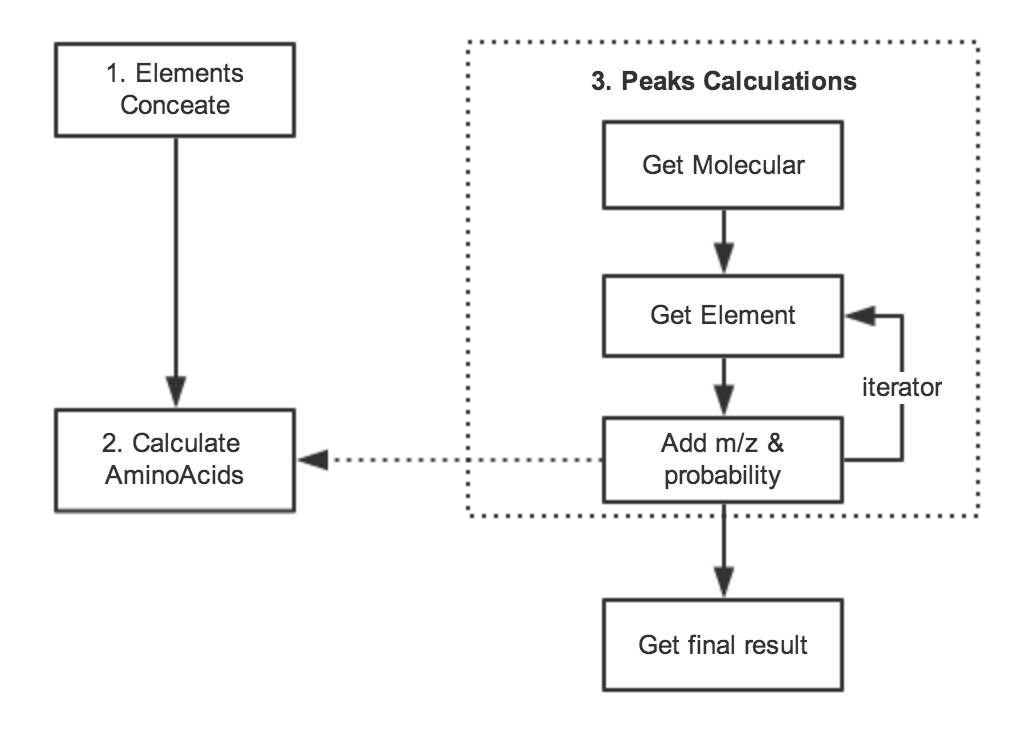
\includegraphics[scale=0.45]{ipc01}
\caption{IPC Process}
\label{threadsVsSync}
\end{figure}

Complexity

There should be several molecular from a protein sequence shear. In general, a 200-250 length sequence will be shear to 800~900 molecular. There also are about 3000 protein sequences in a single file about 14mb. Above all, the complexity is very large.

As for the old algorithm to calculate all of molecular peaks, it is a large Amount of calculation.  The calculation formula of each molecular is below:

$$\sum_{i_1=1}^n (S_1^{2i}) * \sum_{i_2=1}^n (S_2^{2{i_2}}) \cdots  \sum_{i_n=1}^n (S_n^{2{i_n}}) $$

$S_n$ standards the number of isotope for each element. n is the element number in specified molecular. As for this formula, the amount if calculation is totally large which is hard to be calculated out. In order to restraint the amount of calculation, IPC set a calculation threshold which try to limit the number of result list in each calculation step.  When the number is large than this threshold, program will cut result then only keep the top N results according to the threshold number. In IPC origin program, this threshold is set to be 100 so that the formula should change to below:

$$\sum_{i_1=1}^n 200^2 + \sum_{i_2=1}^n 200^2 \cdots \sum_{i_n=1}^n 200^2$$

This limitation can effectively reduce the effort of calculation, besides, it can keep most useful peaks because we don't care many peaks with very low probability. It is hard to contribute the program for protein searching.  With this action, our algorithm can be calculated out in a available time but it still cost to much. 

\begin{figure}[h!]
\centering
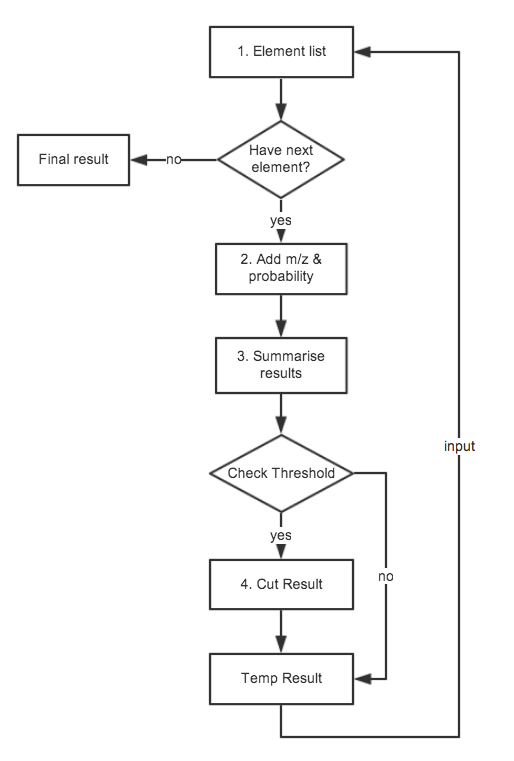
\includegraphics[scale=0.45]{ipc02}
\caption{IPC Process 2}
\label{threadsVsSync}
\end{figure}

The process of IPC is summarised as Figure2.

Step 1. Get list of elements.

In this step, program extract the molecular's element's species and scale then store in data structure. 

Step 2. Add m/z and probability

For each isotope of elements will be added to final results with different peaks which be expressed by a key value pair of m/z value and probability.  So the number of peaks results is decided by the number of isotope of element and the number of elements in specified molecular.

Step 3. Summarise peaks results

Each two peaks result with similar m/z value should be summarised to on peaks with probability of expectation of two peaks probability. In this summary step, the calculation scale is $N^2$ (N is number of peaks results).

Step 4. Cut results

In this step a result should be generated and program will  check if the size of peaks result is large than threshold, if so, program will cut the results and keep top 100 results which sorted by probability from large to small. After this step , process will continue to get next element's isotope and back to Step1 until there no any other element to add.

\begin{figure}[h!]
\centering
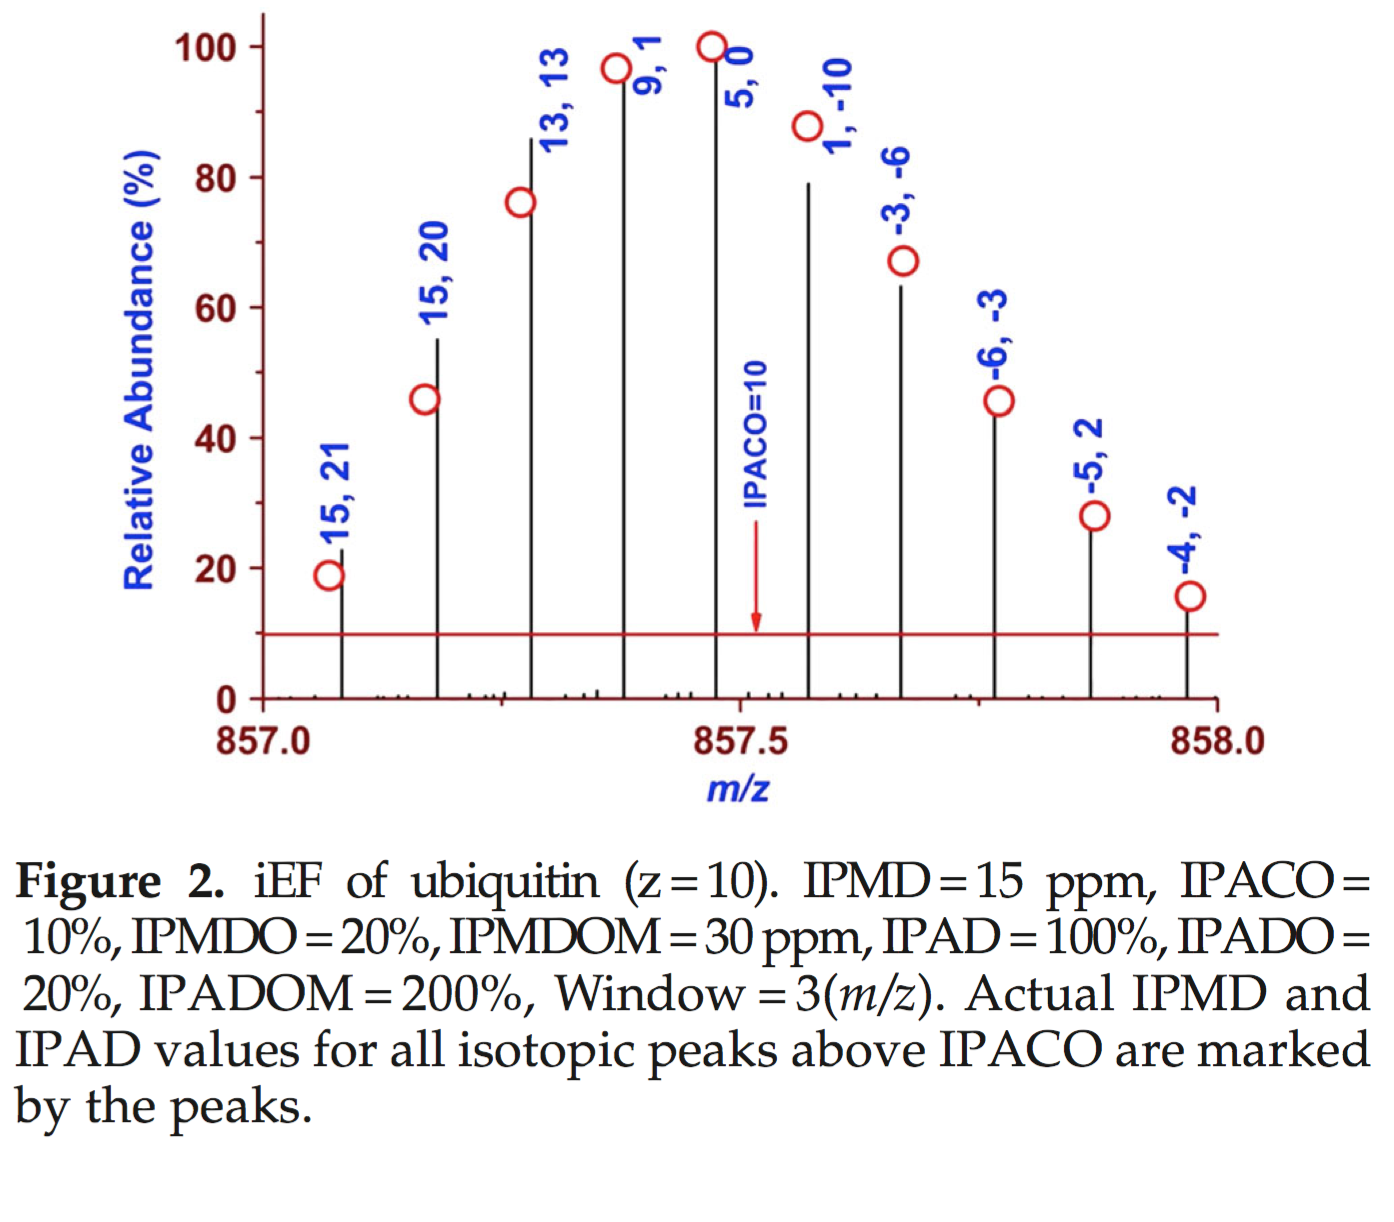
\includegraphics[scale=0.35]{protein01}
\caption{IPC Process}
\label{threadsVsSync}
\end{figure}


\subsection{Limitation}

Firstly, The methodology of IPC to calculate peaks result is very reasonable when calculate a small amount of molecular's peaks but it obviously has much redundant computing when calculate a large amount of molecular.  For each molecular, IPC will add m/z and multiple probability from very beginning to end which means IPC may calculate C1000's peaks at first molecular then calculate C1001's peaks in second peaks but the result of C1000 can't be used to calculate C1001. This is totally waste computing resource when it need to calculate out a long sequences of protein which have many big molecular need be put into peaks calculations. 

Secondly, the calculation for result peaks is serial. Each element's isotope will be add to results one by one so that the process is very  inefficient because there are so much CPU time are wasted during waiting. Especially for a large sequence calculation, this is a bad strategy for process the program as serial.

These two limitations are restrict the application of ProteinGoggle because the time of calculation is too long when meet large protein sequence which is usual in protein experiment. So the methodology of Speed Acceleration comes to very important and meaningful in 
protein searching. 

\section{Methodologies}

We put forward some new strategy to accelerate protein peaks calculation for protein searching.  It contains two parts: (1) Pre-database store; (2) GPU parallel calculation.

\subsection{Pre-database store}

In Section3.3 we have described the limitation of redundant computing which will waste much time during large sequence with many large amount of elements' molecular although IPC set a threshold to reduce the complexity of computing. But it still have so much potential to reduce the computing scale. 

We know that the main elements which composite a protein is always limited although there are so many different molecular in nature.  We can't pre-store all molecular's peaks but we can just store the peaks of single element with any scale which means we can pre-calculate peaks of sole elements of different scale. 

\begin{figure}[h!]
\centering
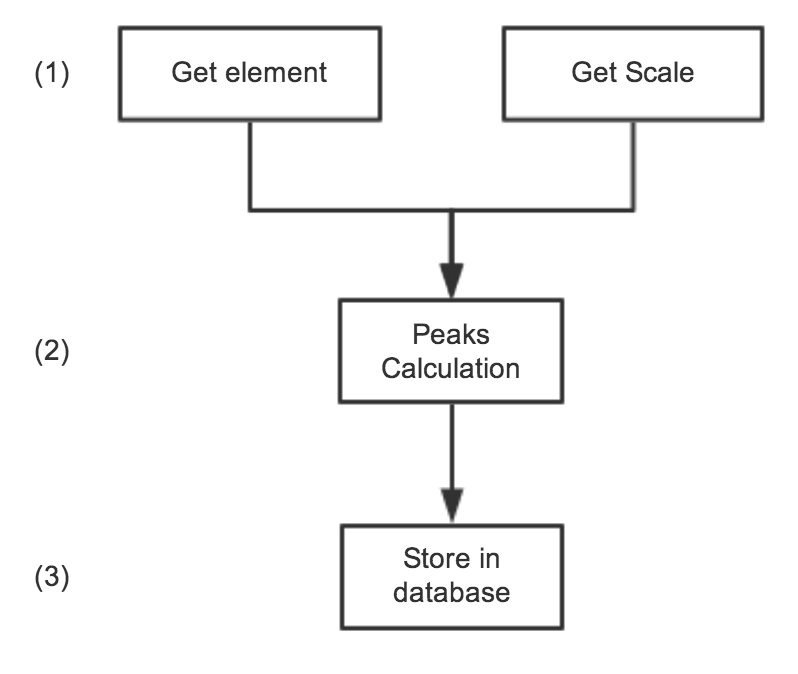
\includegraphics[scale=0.45]{ipc03}
\caption{IPC Process 3}
\label{threadsVsSync}
\end{figure}

As the figure 3 show, for each frequency element, the program will calculate the isotope peaks of sole element with range of scale. This calculation is same with the computing process described in Figure2. In our test environment, we calculate element each element's peaks are summarised as table 1. It is easy to dynamically expand the scale because this is only the sole computing and results can be reused in future.

\begin{center}
\begin{tabular}{c|c|c}
\hline
Element & From & To\\
\hline
C & 1 & 1000\\
\hline
H & 1 & 4000\\
\hline
O & 1 & 500\\
\hline
N & 1 & 400\\
\hline
S & 1 & 30\\
\end{tabular}
\end{center}

With pre-database store of sole element's peaks, the process of IPC core is change to what Figure4 show.

\begin{figure}[h!]
\centering
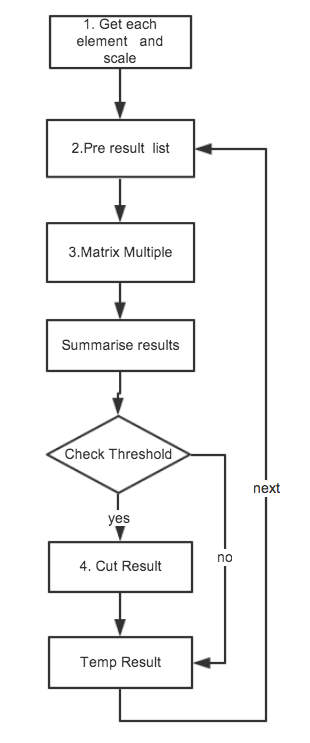
\includegraphics[scale=0.45]{ipc04}
\caption{IPC Process 4}
\label{threadsVsSync}
\end{figure}

Step 1. Get element and scale

Program now will just get each element's type and its maximal scale then store in a data structure. It like a dictionary which standard a molecular's composition of different elements and the number of each element. 

Step 2. Get pre-stored peaks results
 
With the key store in Step 1, we can query and get pre-stored peaks result which we calculated before and store in database. For example, if a molecular is composited by $C_{1000}H_{2000}O{300}N{200}$, the program will query the peaks results of $C_{1000}$, $H_{2000}$,$O_{300}$,$N_{200}$.

Step 3. Matrix Multiple

What we get from in Step 2 are some list of peaks results which contains m/z and probability and we want to get peaks results which are the combinations of them. This is very easy to make each list as a vector and multiple them to get the results we want. 

\begin{center}
$\[ \left( \begin{array}{cc}
mz1 & probability1 \\
mz2 & probability2 \\
\cdots & \cdots \\
mzn & probabilityn \\
\end{array} \right)
* 
 \left(\begin{array}{cc}
mz1 & probability1 \\
mz2 & probability2 \\
\cdots & \cdots \\
mzn & probabilityn \\
\end{array} \right)
\]$
\end{center}

Just as the formula show above, the peaks result will be calculated out by combining each peaks in sole peaks results according to the element type and scale. Then the program also need to summarise similar m/z value peaks and cut result to be a reasonable size.

\subsection{GPU parallel calculation}

Matrix multiple is also a very complex work for normal Centre Process Unit, but it is very each to process when it can be run in GPU. So we put forward a single way to process Matrix Multiple step  in GPU.

GPU(Graphics Processing Unit) has become an integral part of today's mainstream computing systems. Over the past six years, there has been a marked increase in the performance and capabilities of GPUs.The modern GPU is not only a powerful graphics engine but also a highly parallel programmable processor featuring peak arithmetic and memory bandwidth that substantially outpaces its CPU counterpart. The GPU?s rapid increase in both programmability and capability has spawned a research community that has successfully mapped a broad range of computationally demanding, complex problems to the GPU. 

CUDA can facilitate issuing and managing computations on the GPU as a data-parallel computing device without the need of mapping them to a graphics API. Therefore, CUDA provides more flexibility to efficiently map a computing problem onto the hardware architecture.
Programming with CUDA, the GPU is regarded as a compute device which can execute numerous threads in parallel. It can be manipulated as a co-processor to the CPU (host). Each CUDA-compliant device is a set of multiprocessor cores (see Fig.2) and each stream multiprocessor (SM) on GPU is implemented as Single Instruction Multiple Data (SIMD) architecture. That is, each processor of the multiprocessor executes a different thread but all the threads run the same instruction, operating on different data based through the thread Id, at any given clock cycle.

\begin{figure}[h!]
\centering
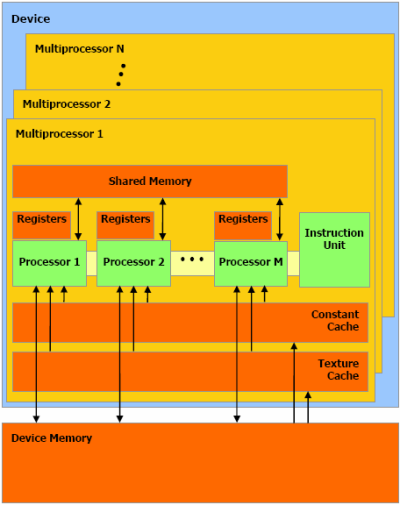
\includegraphics[scale=0.7]{cuda1.png}
\caption{Processors, multiprocessors, and more processors}
\label{threadsVsSync}
\end{figure}


Multiprocessors have on-chip memory that can be of the four following types: registers, shared memory, constant cache and texture cache. Each processor in a multiprocessor has one set of local 32-bit read-write registers per processor. A parallel data cache of shared memory is shared by all the processors. A read-only constant cache is shared by all the processors and speeds up reading from the constant memory. A read-only texture cache is shared by all the processors and speeds up reading from the constant memory. . A read-only texture cache is shared by all the processors and speeds up reads from the texture memory. The local and global memory spaces are implemented as read-write regions of device memory and are not cached.

The batch of threads that execute a kernel is organized as a grid of thread blocks, as shown in Fig. 3. 

\begin{figure}[h!]
\centering
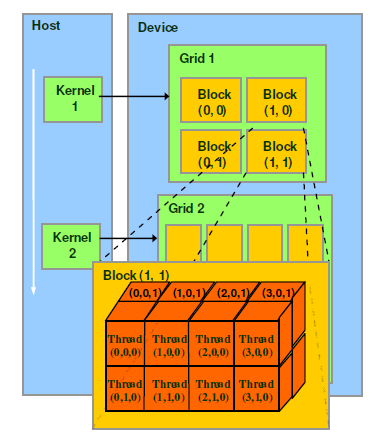
\includegraphics[scale=0.7]{cuda2.png}
\caption{Figure 3. Grid of thread blocks in GPU}
\label{threadsVsSync}
\end{figure}

Threads within a block or a warp can cooperate among themselves by sharing data through shared memory and synchronizing their execution to coordinate memory accesses. Thread blocks are required to execute independently. A thread scheduler periodically switches from one warp to another to maximize the use of multiprocessor?s computational resource.

\subsection{CUDAFY Framework}
CUDAfy .NET allows easy development of high performance GPGPU applications completely from the Microsoft .NET framework. It's developed in C. The old software are based on C so that we have to call GPU calculation program in C runtime environment. CUDAFy is a framework which can support user program in c to call core program of calculation in GPU with CUDA framework. It makes CUDA programming even more convenient than with Nvidia's C-based runtime. 

\subsection{CUDA and matrix multiply}

The matrix of molecular's peaks is a very high dimension data so that the multiple of each item is a time cost operation. But in CUDA, it is easy to calculation the peaks results by parallel way.  The figure X shows the implementation of peaks matrix multiple in CUDA.

\begin{lstlisting}[ language=C] 
int main(int argc, char ** argv) 
{ 

printf("Hello world! \n"); 

return 0; 
} 
\end{lstlisting} 

\section{Evaluation}

Experiment have been performer to accelerate the speed of Protein Isotopic Envelope Fingerprinting  database computing which used to compare the similarity level of mass spectrum. We compared the the implementation of ProteinGoggle in CUDA with:

* The result of former resort was implemented in single PC which is with corei7/8 core cpu.

We have implemented our solution on a workstation which has the xxxx GHz Intel processor, one NVIDIA GT760 graphic cards and 8Gb memory. The former programs are written in c which support easy-use GUI for most of users. In order to make the performance Optimization as simple as we can, we just change the core algorithm and strategy of calculation in our new program which based on GPU calculation in CUDA framework.

We have run test with a 200-250 sequence size protein file with is as large as 14mb. In former strategy and workload, it will cost about 13 days in database calculation. 

With our new strategy and algorithm, it only costs about 1.5 hours. This result are tested in our workstation which described before. 

For more details, the diagram shows the performance tracks:

\section{Conclusion}

\subsection{Future Work}


\theendnotes
\end{document}







